\section{\SysName}

\begin{figure}[tb]
    \centering
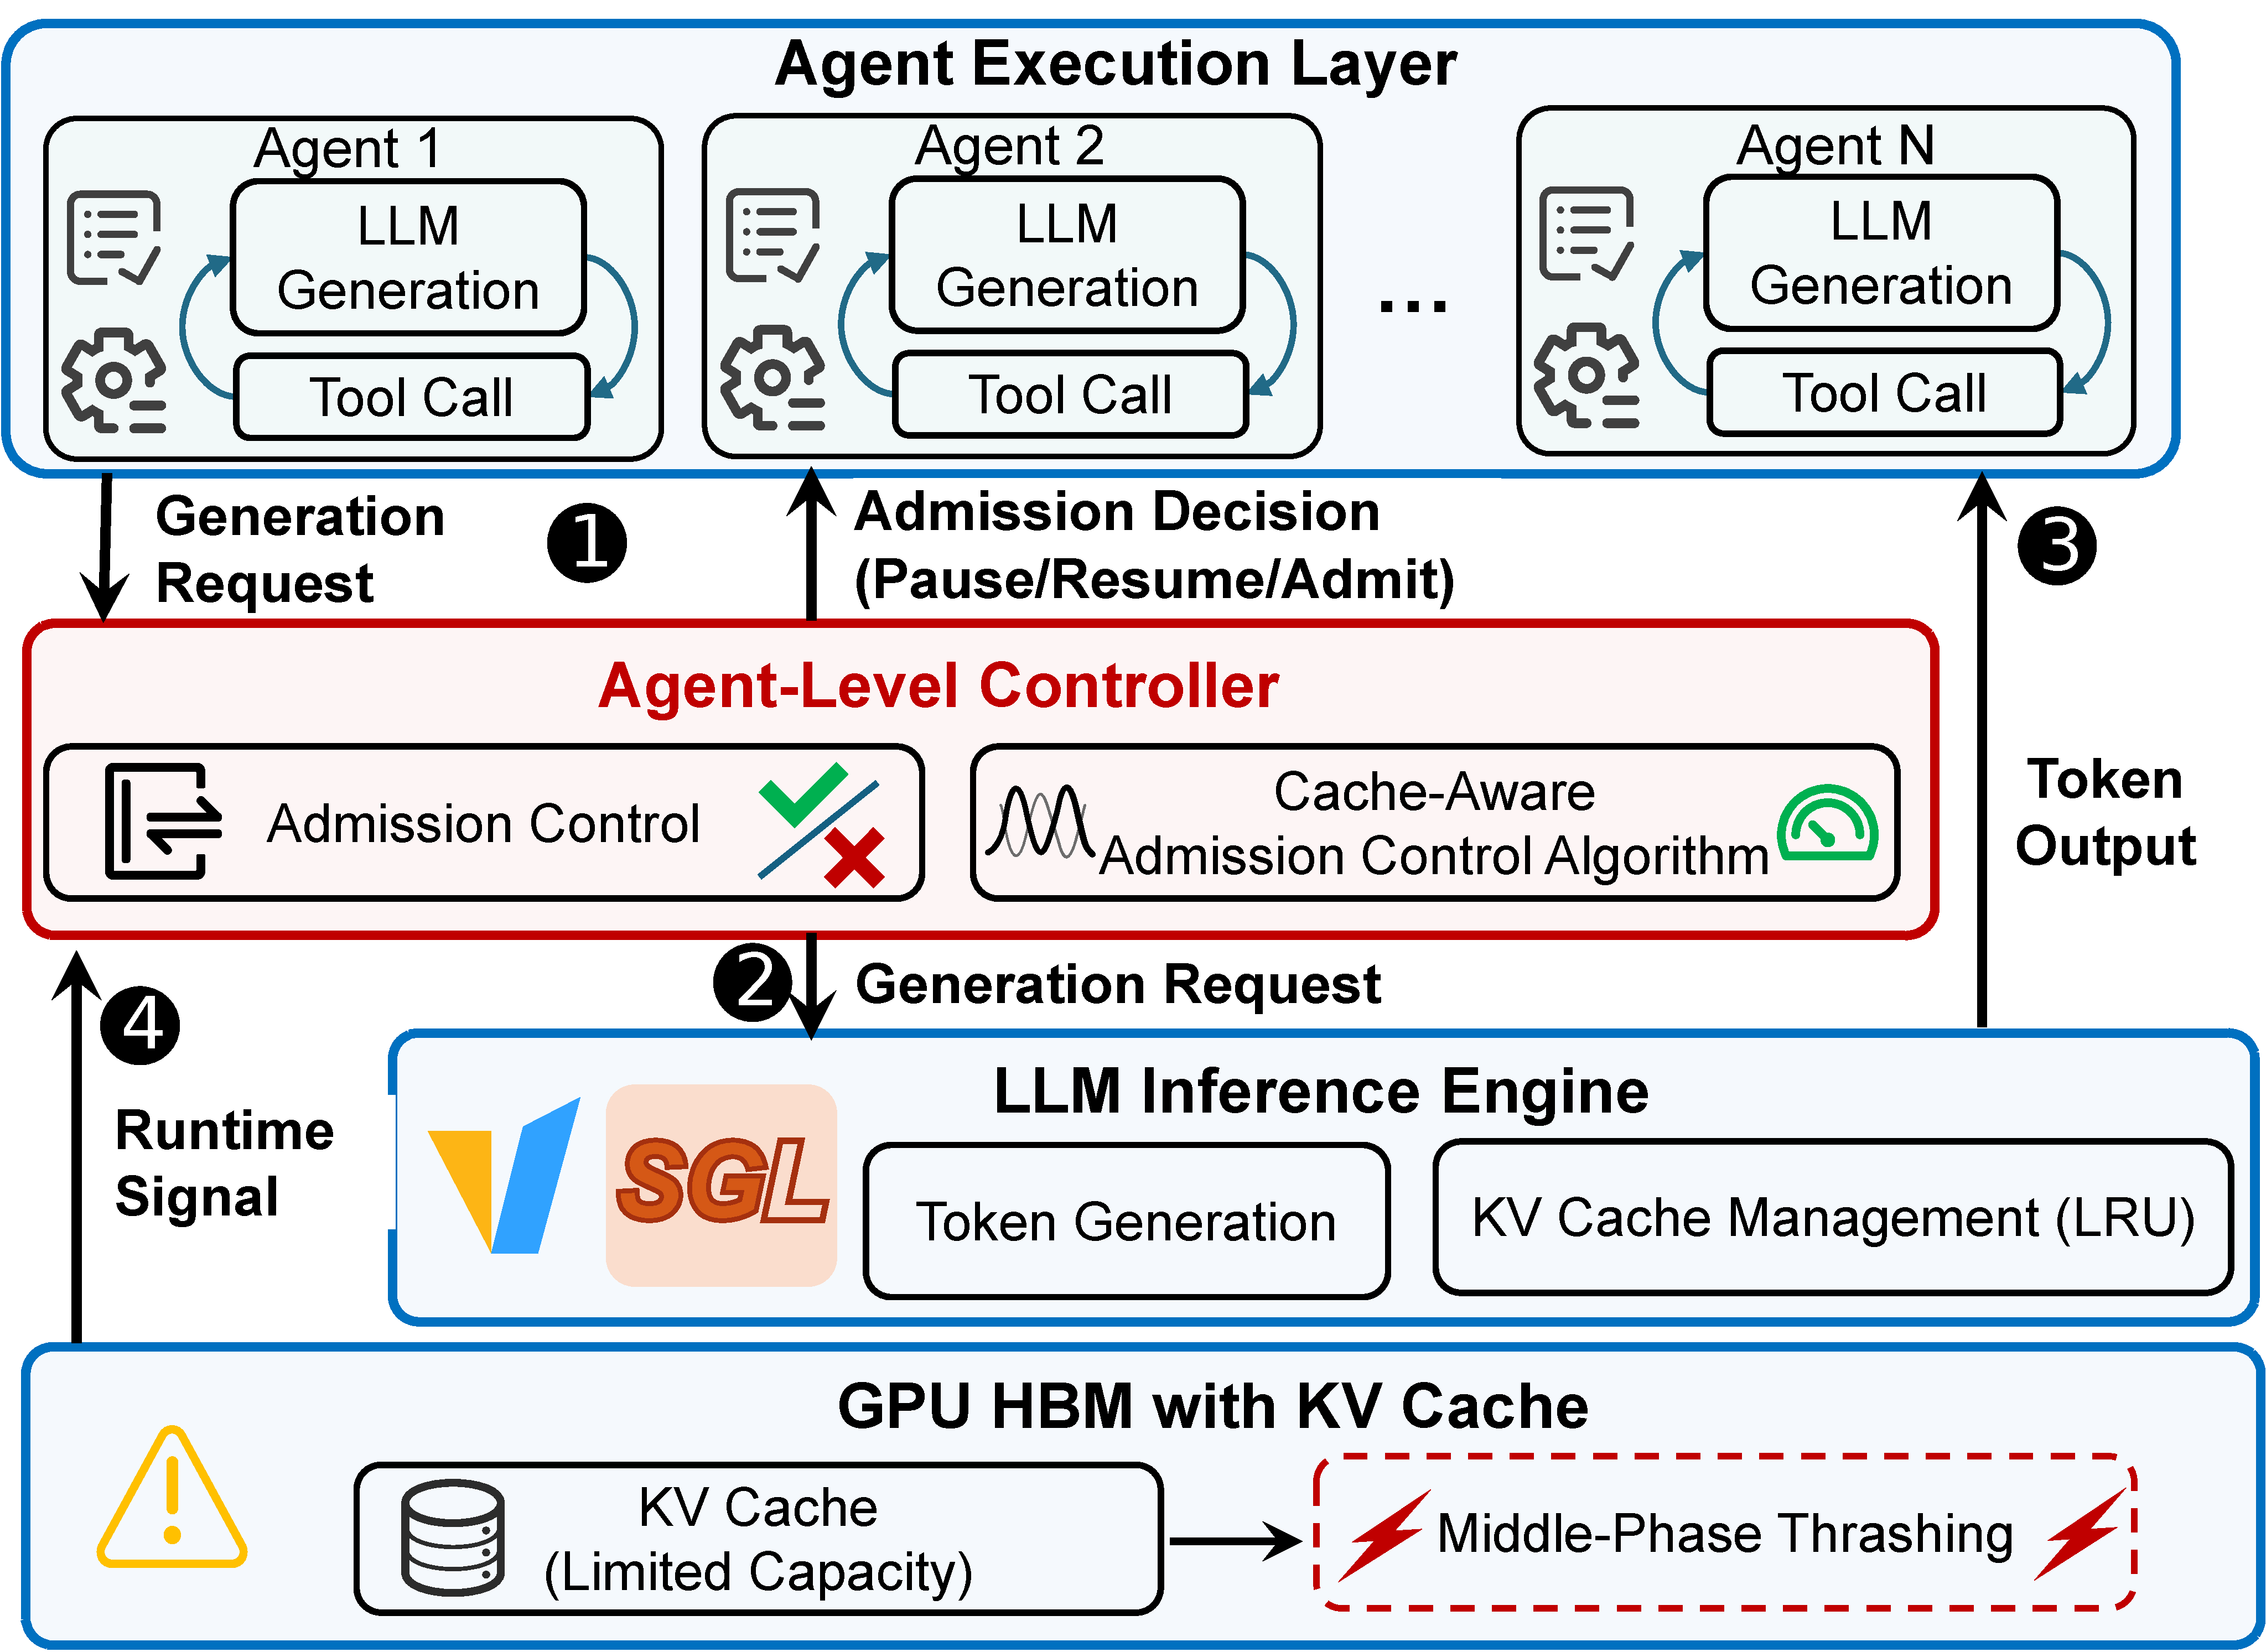
\includegraphics[width=0.98\linewidth]{figure/SystemOverview.pdf}
    \caption{系统概览。}
    \label{fig:systemoverview}
\end{figure}

\subsection{系统概览}
图~\ref{fig:systemoverview} 展示了 \SysName{} 所处的系统上下文。我们的设计并不试图重新实现一套端到端服务栈，而是在现有 Agent 执行框架与 LLM 服务引擎之间\emph{插入一个轻量级的 Agent 级控制器}。整体系统可以概念性地分为三部分：Agent 执行层、Agent 级控制器和 LLM 服务引擎。

(1) \textbf{Agent 执行层。}
位于系统顶层，多个 Agent 按照 ReAct 风格循环执行长时程工作流。

(2) \textbf{LLM 服务引擎。}
LLM 服务引擎（例如 SGLang）负责 token 生成，并管理 GPU 显存中的 KV 缓存。

(3) \textbf{Agent 级控制器。}
为了缓解中期抖动，这个控制器在\emph{Agent 粒度}上执行准入管理。与请求级调度器不同，它在多个生成步骤之间保留 Agent 的连续性。控制器持续监测实时 KV 缓存使用率与命中率，并动态调节整体活跃 Agent 并发度，以防止\emph{中期抖动}。

\noindent\textbf{执行流程。} 整个系统通过四个阶段形成闭环。
\circled{1} \textbf{Agent 准入。}
Agent 在需要执行生成步骤时，不再直接向服务引擎发起请求，而是先提交给控制器。控制器根据当前系统状态决定准入还是暂停，并保留其执行状态。
\circled{2} \textbf{批量生成。}
被准入的 Agent 在服务引擎中进行批量 token 生成，并按照上下文长度消耗 GPU 驻留 KV 缓存。
\circled{3} \textbf{工具执行与挂起。}
调用外部工具的 Agent 会暂时变为不活跃，但它们在逻辑上仍保有与自身关联的 KV 状态。控制器通过在高压力阶段限制新的准入，尽量保护这些空闲状态不被淘汰。
\circled{4} \textbf{反馈与控制更新。}
控制器持续采集运行时信号，尤其是 KV 缓存使用率与命中率，并据此按 \S\ref{subsec:AIMD} 中的自适应机制更新准入策略，从而在维持吞吐的同时避免抖动。

\subsection{Agent 级控制器}
离线 Agent 批量推理的核心挑战在于：Agent 具有长生命周期、强状态性的执行语义，而现有 LLM 服务引擎通常基于请求中心抽象。为弥合这一差距，我们引入一个\emph{Agent 级控制器}，在 Agent 粒度而非单次生成请求粒度上调节对服务引擎的访问。

Agent 级控制使系统能够围绕并发活跃 Agent 的整体工作集进行推理，而不只是围绕零散请求做局部决策。与其在内存压力出现后再靠缓存淘汰或重计算进行补救，控制器可以主动限制某一时刻允许执行生成步骤的 Agent 数量。这样便能让总 KV 工作集始终保持在 GPU 显存容量之内，从而直接避免中期抖动的出现。

\noindent\textbf{主动准入控制。}
控制器实现了一套主动准入机制。当 Agent 准备执行生成步骤时，它会先把请求提交给控制器，而非直接进入服务引擎。控制器根据当前系统条件决定是否准入。被准入的 Agent 进入服务引擎并参与批量生成；未被准入的 Agent 则在 Agent 粒度上暂时暂停，同时保留其执行状态。

图~\ref{fig:twoagent}b 给出了一个 Agent 级准入控制示例。开始时，控制器只允许 A1 和 A2 进入，使它们能够持续被推理引擎调度，同时保证二者组合后的 KV 工作集仍处于 GPU 显存预算之内。其他 Agent（如 A3）则保持等待状态，不发起推理请求，以避免 KV 缓存过量承诺。当 A2 完成执行并释放 KV 缓存后，控制器再从待执行队列中准入 A3。于是，系统始终维持至多两个活跃 Agent，从而保证内存使用稳定并避免由淘汰导致的重计算。

\subsection{缓存感知的准入控制算法}
\label{subsec:AIMD}

对 Agent 工作负载而言，静态准入上限在根本上是不够的。首先，Agent 的内存占用并非固定值，而是随着执行推进单调增长；一个在早期阶段安全的并发上限，迟早会在上下文拉长后触发显存饱和。其次，Agent 的推进是异步的，生成与外部工具执行交替出现，即使 Agent 总数不变，聚合内存需求也会不可预测地波动。因此，系统面临两难：过于保守的静态上限会浪费宝贵的 GPU 显存，而过于激进的上限则会跨越饱和阈值，进入抖动区间。为了在高利用率和防止抖动之间取得平衡，系统需要一个可以持续跟踪有效容量变化的动态机制。

我们将并发 Agent 的调度形式化为一个在严格内存约束下的资源分配问题，并将其与 TCP 拥塞控制进行对应。在这一类比中，共享 KV 缓存相当于网络带宽，而活跃 Agent 则是争用该有限资源的独立数据流。

\noindent\textbf{问题建模。}
我们将 Agent 执行动态映射为如下的流量控制要素：
\begin{itemize}[nosep]
    \item[(1)] \textbf{拥塞窗口（$W_t$）} 对应于当前允许并发执行的活跃 Agent 数。
    \item[(2)] \textbf{丢包} 对应于\emph{缓存淘汰}，即服务引擎因显存饱和而被迫丢弃活跃上下文。
    \item[(3)] \textbf{重传} 对应于\emph{KV 缓存重计算}。
\end{itemize}

\noindent\textbf{算法设计。}
基于经典 TCP 中的 AIMD 算法，我们提出\emph{缓存感知的准入控制}算法。它依据来自服务引擎的两个实时反馈信号调节窗口大小 $W_t$：其一是\emph{KV 缓存使用率}（$U_t$），作为前瞻性的拥塞信号；其二是\emph{缓存命中率}（$H_t$），作为反应式的失败信号。控制律定义如下：
\begin{equation}
W_{t+1} = \begin{cases}
    W_t + \alpha & \text{if } U_t < U_{low} \\
    W_t \times \beta & \text{if } U_t > U_{high} \land H_t < H_{thresh} \\
    W_t & \text{otherwise}
\end{cases}
\end{equation}

\noindent\textbf{解释。}
该控制律中的每一项都对应 Agent 执行中的一种关键动态：

\begin{enumerate}[leftmargin=*,nosep]
    \item[(1)] \textbf{线性探索（$\alpha$）。}
    当系统处于低利用状态（$U_t < U_{low}$）时，采用加性增大方式线性探测未知的有效容量。这样既能提升 GPU 显存利用率，也能避免指数式放大带来的突然过冲。

    \item[(2)] \textbf{降低二次代价（$\beta$）。}
    与网络中的丢包不同，缓存抖动引发的代价是凸性的，因为重计算随上下文长度增长而非常昂贵。因此，一旦检测到抖动，控制器会执行乘性缩减，使系统能以指数速度退出高代价区域，从而压低累计重计算开销。

    \item[(3)] \textbf{稳定与饱和。}
    $U_{low}$ 与 $U_{high}$ 之间的区间充当了资源分配缓冲区。由于长上下文 Agent 的准入往往会造成离散式显存突增，而非平滑变化，因此该缓冲区可以避免系统因单次突增而立即跌入惩罚状态（$U_t > U_{high}$）。同时，只要命中率仍保持健康，系统就可以在饱和区维持较高并发，以优先保证吞吐。
\end{enumerate}

\noindent\textbf{Agent 级控制原语。}
为了在不与请求级调度强耦合的前提下调节 Agent 执行，控制器暴露了三个最小化的 Agent 级原语：\emph{admit}、\emph{pause} 与 \emph{resume}。它们作用于 Agent 生命周期，而不是单次生成请求。具体而言，\emph{admit} 允许 Agent 执行下一次生成；\emph{pause} 在保留其执行状态的同时，暂时阻止其继续发起请求，并且只会在生成步骤与工具执行之间这类明确边界处生效，以避免打断正在进行的计算；\emph{resume} 则在资源重新可用时恢复一个已暂停 Agent 的执行，并且由准入控制统一协调，避免重新激化缓存拥塞。通过 \emph{pause} 与 \emph{resume}，控制器能够在工作负载变化时动态调整活跃 Agent 集合。
